\documentclass[11pt]{article}
\usepackage[margin=1.1in]{geometry}
\usepackage{amsmath,amssymb,booktabs,graphicx,natbib,hyperref,setspace,multirow}
\usepackage[T1]{fontenc}
\usepackage{url}
\urlstyle{tt}
\Urlmuskip=0mu plus 1mu  % let long URLs breathe in footnotes

% Tables that exceed the text block get scaled; the rest are left alone. The
% width is measured by LaTeX rather than estimated beforehand, so this keeps
% working when the numbers change and a column gets wider.
\newsavebox{\tblbox}
\newcommand{\fittable}[1]{%
  \savebox{\tblbox}{\input{#1}}%
  \ifdim\wd\tblbox>\textwidth
    \resizebox{\textwidth}{!}{\usebox{\tblbox}}%
  \else
    \usebox{\tblbox}%
  \fi
}
\bibliographystyle{plainnat}
\hypersetup{colorlinks=true,linkcolor=black,citecolor=black,urlcolor=blue}
\setlength{\parskip}{2pt}
\emergencystretch=1.5em  % absorb the odd unbreakable citation
\onehalfspacing

\title{\textbf{The Rotation of the Curve:\\ ECB Policy Transmission Before and After\\ Balance Sheet Normalisation}}
\author{Philip Kroos\thanks{\raggedright \href{mailto:philip.kroos@web.de}{philip.kroos@web.de}. Replication code and data
are available at \url{github.com/Philip-Kroos/ecb-surprise-bund-curve}. All errors
are my own.}}
\date{\today}

\begin{document}
\maketitle

\begin{abstract}
\noindent I use intraday asset price changes around 83 ECB Governing Council
meetings between January 2015 and October 2025 to ask whether the transmission
of monetary policy surprises to the German yield curve changed when the euro
area moved from balance sheet expansion to normalisation. Decomposing each
meeting into orthogonal target, path and balance-sheet surprises, I find that
the transmission did not weaken uniformly. It rotated. The balance-sheet factor
transmits with a stable coefficient near unity across both regimes. What changed
is the long end of the curve: a hawkish path surprise lowered thirty-year Bund
yields by 1.30 basis points per basis point before 2022 and has no detectable
effect since, a shift of 1.35 basis points with a wild-bootstrap $p$ value of
0.037. In parallel, target surprises acquired a slope effect they previously
lacked, flattening the two-to-ten segment by 1.46 basis points per basis point
against essentially zero before. The share of meetings on which yields and
equities co-move, the signature of a central bank information shock, fell from
46 to 15 percent. In a four-country panel, target surprises transmit 2.40 basis
points more strongly to periphery than to core ten-year yields, but that
amplification is confined to the expansion regime and disappears after July
2022. Two caveats discipline the reading. Joint stability tests do not reject
coefficient constancy in any single equation, and no individual interaction
survives a family-wise correction across the twenty-one tests examined; the
evidence for the rotation is a consistent pattern of point estimates across
maturities, classifications and robustness variants rather than a decisive
rejection. Taken at face value, the estimates imply that curve sensitivities
calibrated on the quantitative easing period misstate the current reaction, and
that the misstatement is concentrated in the long-duration positions for which
it matters most.

\vspace{1em}
\noindent \textbf{Keywords:} monetary policy transmission, high-frequency
identification, yield curve, quantitative tightening, euro area

\noindent \textbf{JEL:} E43, E52, E58, G12
\end{abstract}

\newpage

\section{Introduction}

Between 2015 and 2021 the European Central Bank operated at the effective lower
bound on its policy rate and conducted policy primarily through asset purchases
and forward guidance. Since July 2022 it has raised and then lowered policy
rates through a full cycle while allowing its balance sheet to contract. The two
configurations differ not only in the stance they delivered but in the
instruments through which the stance was communicated.

This paper asks whether the mapping from policy surprises to the German
sovereign curve changed with that configuration. The question is of interest for
two distinct reasons. For the analysis of transmission, the stability of the
mapping is informative about whether the channels through which asset purchases
and guidance operate are structural or specific to the environment in which they
were deployed. For the practice of fixed income risk management, the mapping is
the object being estimated whenever a desk asks how far the curve will move on a
policy surprise of given size, and a mapping estimated on a regime that has ended
is a source of miscalibration rather than information.

The identification follows the high-frequency event-study tradition
\citep{kuttner2001,gurkaynak2005,altavilla2019}. Within a window of minutes
around a scheduled announcement, the probability that an unrelated macroeconomic
release moves the curve is small, so the observed price change can be attributed
to the announcement. The euro area affords an additional advantage exploited by
\citet{altavilla2019}: the rate decision and the elaboration of the outlook and
the balance sheet are released at separate times, so the two can be separated by
construction rather than by assumption.

I make three contributions. First, I extend the regime comparison to a sample
that contains the complete tightening and partial easing cycle through October
2025, which was not available to the literature that established the baseline
estimates. Second, I test explicitly whether the response coefficients are
constant across the two regimes, using inference calibrated to the small number
of post-liftoff meetings rather than relying on asymptotic approximations that
are known to over-reject. Third, I show that the change in the mapping is a
rotation of the curve response rather than an attenuation, and I trace the
rotation to two specific coefficients.

The main results can be stated compactly. The balance-sheet factor moves the
Bund curve roughly one for one at every maturity, and this is true in both
regimes; the interaction terms are small and never approach significance. The
change is concentrated in the path factor at the long end and in the target
factor's effect on the slope. Before 2022 a hawkish path surprise lowered
ten-year and thirty-year Bund yields, an inversion consistent with guidance that
signals a lower expected terminal rate or a weaker growth path. That response is
gone. Meanwhile target surprises, which had no discernible effect on the slope
during the expansion, now flatten the curve substantially.

The paper also documents two auxiliary findings that bear on interpretation. The
fraction of meetings on which the equity market moves with rather than against
the interest rate surprise, the sign signature of the central bank information
effect of \citet{jarocinski2020} and \citet{nakamura2018}, falls by two thirds
between the regimes. And the differential transmission of policy surprises to
periphery sovereign yields, which was large and precisely estimated during the
expansion, is absent afterwards.

\begin{figure}[htbp]\centering
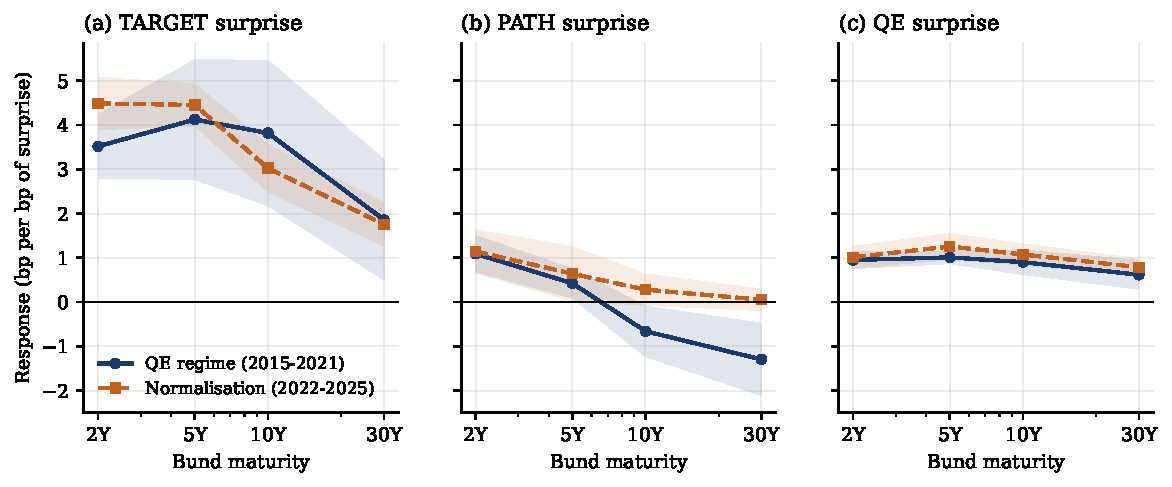
\includegraphics[width=\textwidth]{../output/figures/fig3_curve_response.pdf}
\caption{\textbf{The result in one picture.} Response of Bund yields to each
policy surprise, by regime, with 90 percent confidence bands. The balance-sheet
factor (right) is unchanged across regimes. The path factor (middle) lowered
long yields before 2022 and does not now. Coefficients are basis points of
yield change per basis point of surprise in each factor's anchor instrument.}
\label{fig:curve}
\end{figure}

Section \ref{sec:background} sets out the institutional timeline and states the
hypotheses. Section \ref{sec:data} describes the data. Section
\ref{sec:identification} develops the identification. Section
\ref{sec:results} reports results, Section \ref{sec:portfolio} translates them
into portfolio arithmetic, Section \ref{sec:robustness} reports robustness, and
Section \ref{sec:conclusion} concludes with the limitations that a reader should
weigh against the findings.

\section{Institutional background and hypotheses}
\label{sec:background}

The sample opens with the announcement of the expanded asset purchase programme
on 22 January 2015 and closes on 30 October 2025. Three features of the interval
matter for the design.

Until July 2022 the deposit facility rate was at or below zero and unchanged for
long stretches. Policy news therefore arrived predominantly as information about
the pace and duration of purchases and about the conditions under which rates
would eventually rise. On 21 July 2022 the Governing Council raised rates for the
first time in eleven years and simultaneously announced the Transmission
Protection Instrument. Net purchases under the asset purchase programme had ended
the preceding month, and portfolio runoff began in March 2023.

I therefore define an expansion regime through December 2021 and a normalisation
regime from July 2022, and treat the first half of 2022 as a transition that the
baseline excludes and the robustness section restores. The exclusion is a
judgement, not a result, and Section \ref{sec:robustness} shows the findings do
not depend on it.

Five hypotheses were fixed before estimation.

\textbf{H1, segmentation.} Target surprises move the short end most, path
surprises the short to intermediate segment, and balance-sheet surprises the long
end.

\textbf{H2, attenuation.} The long-end response to balance-sheet surprises is
weaker in the normalisation regime, because portfolio runoff is passive,
pre-announced and calendar-based, and therefore carries less surprise per meeting
than the discretionary purchase announcements whose duration-extraction
effects the earlier literature documents \citep{krishnamurthy2011,rogers2014}.

\textbf{H3, slope.} Restrictive target surprises flatten the curve; restrictive
balance-sheet surprises do not.

\textbf{H4, information.} A material share of meetings are information rather
than policy shocks, and removing them sharpens the estimated responses.

\textbf{H5, fragmentation.} Balance-sheet surprises transmit more strongly to
periphery than to core sovereign yields.

H2 and H5 are rejected in the forms stated. I report them as stated rather than
revising them after the fact, because the informational content of a rejected
prior differs from that of a hypothesis constructed to fit.

\section{Data}
\label{sec:data}

The source is the Euro Area Monetary Policy Event-Study Database of
\citet{altavilla2019}, maintained by the ECB. It records intraday changes in
overnight index swap rates from one month to twenty years, sovereign yields for
Germany, France, Italy and Spain, the EURO STOXX 50 and its banking subindex, and
major euro exchange rates, separately for the press release window, the press
conference window and their union.

Restricting to meetings from January 2015 yields 83 events, 56 in the expansion
regime and 27 in the normalisation regime. All series used below are complete
over this interval. Yield changes are in basis points and equity changes in
percent.

\paragraph{A cleaning step that is not innocuous.} The distributed workbook
stores the event date as a native date for early observations and as a
\texttt{dd/mm/yyyy} text string for later ones. A reader applying month-first
conventions to the text rows transposes day and month whenever both are below
thirteen. In the current vintage this mis-assigns six dates, every one of them in
2024 or 2025, and therefore falls entirely within the regime whose coefficients
are the object of the exercise. Each mis-parsed date is placed on a Sunday,
Monday or Tuesday, whereas all Governing Council monetary policy meetings in the
sample fall on a Wednesday or Thursday, which provides a simple diagnostic. The
replication code parses the raw cells by type and verifies the day-of-week
distribution. Appendix Table A1 lists the affected dates. I record this not for
its intrinsic interest but because it is invisible in any output that does not
inspect the calendar, and because the errors concentrate precisely where the
paper's identification of a regime change requires them not to.

\section{Identification}
\label{sec:identification}

\subsection{The event window}

Let $\Delta p_t$ denote the change in an asset price across the announcement
window on meeting date $t$. The identifying assumption is that, conditional on
being in the window, no news other than the announcement moves the price:
\begin{equation}
\Delta p_t = \Gamma' s_t + \varepsilon_t, \qquad E[s_t \varepsilon_t] = 0,
\end{equation}
where $s_t$ collects the policy surprises. Two threats deserve statement rather
than assertion. Macroeconomic releases scheduled inside the window would violate
the exclusion; euro area releases are not scheduled during Governing Council
windows, though US releases occasionally are, which motivates the control in
Section \ref{sec:robustness}. And complex balance-sheet announcements may be
priced with a lag exceeding the window, which would attenuate the balance-sheet
coefficients toward zero. Attenuation of this kind biases against finding the
stable balance-sheet transmission reported below only if it worsened over time,
for which there is no evident reason.

\subsection{Factor decomposition}

A single meeting conveys several pieces of news at once, so a scalar surprise
measure confounds them. Following \citet{gurkaynak2005}, \citet{swanson2021} and
\citet{altavilla2019}, I extract orthogonal factors and rotate them into
economically interpretable positions.

Write the matrix of OIS surprises in a given window as $X = F \Lambda' + e$ with
$F'F/n = I_k$. In the press release window a single component accounts for 68.4
percent of the covariation; I label it \textsc{target}. In the press conference
window the first two components account for 90.7 and 5.9 percent, so I set
$k = 2$ and rotate by an orthonormal $R$ obtained as the matrix exponential of a
skew-symmetric matrix, which enforces orthonormality at every point of the
optimisation. The single restriction
\begin{equation}
\left[\Lambda R\right]_{\text{1M},\,\textsc{qe}} = 0
\end{equation}
just identifies the rotation angle: the balance-sheet factor is the linear
combination that leaves the one-month OIS unchanged. The residual dimension is
labelled \textsc{path}.

Because $R$ is orthogonal, the rotation relabels variation without creating or
destroying it. The decomposition is a measurement device, not a structural
model, and nothing below should be read as identifying deep parameters.

\paragraph{Scaling.} Each factor is scaled so that a one-unit realisation moves
its anchor instrument by one basis point: the one-month OIS for \textsc{target},
the two-year for \textsc{path}, the ten-year for \textsc{qe}. Every coefficient
reported below is therefore read as basis points of Bund yield change per basis
point of surprise in the anchor. This step is easy to omit and its omission
renders the magnitudes uninterpretable.

Figure \ref{fig:loadings} shows the resulting loading profiles. They have the
shapes the labels imply and were not imposed: \textsc{path} peaks between one and
two years and decays to zero by ten, \textsc{qe} rises monotonically from zero at
one month to unity at the long end.

\subsection{Regime specification}

The estimating equation is
\begin{equation}
\Delta y_t^{(\tau)} = \alpha + \delta\, QT_t
+ \sum_{k} \left(\beta_k + \gamma_k\, QT_t\right) F_{k,t} + \varepsilon_t,
\label{eq:main}
\end{equation}
where $QT_t$ indicates the normalisation regime. The $\gamma_k$ are the objects
of interest.

\paragraph{Inference.} With 27 events in the normalisation regime, asymptotic
inference on $\gamma_k$ is the weakest link in the design. I therefore report,
alongside HC1 standard errors, $p$ values from a restricted wild bootstrap in the spirit of \citet{cameron2008}:
residuals are drawn from the model estimated under $H_0: \gamma_k = 0$,
perturbed by Rademacher weights, and the $t$ statistic is recomputed 4{,}999
times. Where the two disagree I defer to the bootstrap, and I flag the cases
where they do.

\subsection{Separating policy from information}

A restrictive surprise accompanied by rising equity prices is difficult to read
as pure tightening. Following the logic of \citet{jarocinski2020} and
\citet{nakamura2018}, I classify a meeting as a policy shock when the two-year
OIS surprise and the EURO STOXX 50 response have opposite signs and as an
information shock when they agree. This sign classification is coarser than a
sign-restricted vector autoregression and assigns events near the axes on weak
evidence, but it requires no auxiliary model and can be verified by inspecting
Figure \ref{fig:information}.

\section{Results}
\label{sec:results}

\subsection{Baseline responses}

Table \ref{tab:baseline} reports the pooled specification. All three factors move
the curve and the pattern is broadly consistent with H1. Target surprises
generate the largest movements, peaking between two and five years at roughly
4.2 basis points per basis point of one-month OIS surprise and declining to 1.8
at thirty years. Path surprises move the two-year point by 1.17 and have no
average effect beyond ten years. The balance-sheet factor moves every maturity by
close to unity.

Level, slope and curvature are the empirical curve summaries of
\citet{dieboldli2006}; using them avoids fitting a parametric curve to a
four-point cross-section. The last observation qualifies H1. The balance-sheet factor is not a long-end
factor in its effect on Bunds; it is a level factor. This is not mechanical.
The factor is anchored on the ten-year OIS, so unity at ten years is imposed, but
unity at two years is not.

\subsection{The regime comparison}

Table \ref{tab:interaction} contains the paper's central result and Figure
\ref{fig:curve} displays it. The table reports the four outcomes the discussion
turns on; Appendix Table A3 adds the remaining three.

The balance-sheet factor is stable. Its interaction with the regime dummy is
between 0.06 and 0.25 across maturities, never significant at conventional levels
under either inference method, and of the opposite sign to that predicted. H2 is
rejected. Whatever else changed with normalisation, the pass-through from
balance-sheet news to the German curve did not.

Two coefficients did change. The response of long Bunds to path surprises moved
from $-0.66$ (s.e.\ 0.35) to $+0.28$ (0.22) at ten years, an interaction of
$0.94$ with bootstrap $p = 0.064$, and from $-1.30$ (0.50) to $+0.05$ (0.15) at
thirty years, an interaction of $1.35$ with bootstrap $p = 0.037$. During the
expansion, a hawkish path surprise reliably lowered long yields. The response is
now indistinguishable from zero.

Second, the slope. Target surprises had no effect on the two-to-ten segment
during the expansion ($0.30$, s.e.\ 0.81). They now flatten it by $1.46$ basis
points per basis point, an interaction of $-1.76$ with bootstrap $p = 0.033$.

How strong is this evidence taken as a whole? Table \ref{tab:stability}
reports, for each equation, a joint Wald test of the null that all three
interaction coefficients are zero, with a bootstrap distribution generated under
the stable-coefficient null. The test does not reject anywhere; the smallest
$p$ value is 0.165 at thirty years. Likewise, none of the twenty-one individual
interactions survives a Holm correction across the full set: the two headline
$p$ values of 0.033 and 0.037 rise above 0.68 once the family is accounted for.
The honest summary is therefore not that a structural break is established.
It is that the point estimates move coherently, in the same direction, across
maturities, across the shock classification and across every robustness variant
in Section \ref{sec:robustness}, while the sample is too short for any single
test to settle the matter. Figure \ref{fig:rolling} makes the same point
without a test: the rolling path coefficient drifts from negative territory to
zero across the transition rather than jumping, which is what a gradual change
in the information content of guidance would produce and what a 27-meeting
subsample cannot sharply date.

Taken together the two shifts describe a rotation. Policy news that arrives
through rates and guidance is now absorbed at the front end and transmitted into
curve shape, whereas during the expansion it propagated to the long end and
inverted it. The plain reading is that guidance about the near-term path no
longer carries information about the terminal rate or the growth outlook in the
way it did when rates were pinned at the lower bound and guidance was the
principal instrument.

\subsection{Information shocks}

Table \ref{tab:shocks} and Figure \ref{fig:information} report the
classification. Information shocks account for 46.4 percent of expansion-regime
meetings and 14.8 percent of normalisation meetings. The interpretation is not
that the ECB stopped conveying information about the economy, but that its
announcements are now read predominantly through the policy channel.

Re-estimating on the 53 policy shocks sharpens one result and weakens the other.
The slope result strengthens: the target interaction becomes $-1.53$ with
bootstrap $p = 0.019$. The long-end path result attenuates to $0.66$ at ten
years with $p = 0.111$ and $1.09$ at thirty years with $p = 0.161$. Part of the
long-end shift therefore operates through meetings that convey information about
the outlook rather than about the stance. H4 is supported in the weak sense that
the classification matters; it is not the case that removing information shocks
uniformly sharpens the estimates.

\subsection{Cross-country transmission}

Table \ref{tab:panel} reports the four-country panel with unit fixed effects and
date-clustered standard errors. At ten years, target surprises transmit 2.40
basis points more strongly to Italian and Spanish yields than to German and
French ones ($p = 0.009$). The balance-sheet factor shows no differential
($-0.09$, $p = 0.548$). H5 is rejected as stated: fragmentation in this sample is
a rate-surprise phenomenon, not a balance-sheet phenomenon.

The spread regressions in Table \ref{tab:spreads} add the regime dimension and
are the sharpest result in the paper. During the expansion, a one basis point
target surprise widened the Italian ten-year spread over Bunds by 15.7 basis
points. The regime interaction is $-13.6$ with bootstrap $p = 0.033$, leaving a
residual effect of about 2.1 that is not distinguishable from zero. The pattern
repeats for Spain and, more weakly, for France. The sensitivity of periphery
spreads to policy rate surprises has effectively vanished.

The timing invites a conjecture. The Transmission Protection Instrument was
announced on 21 July 2022, the same meeting at which rates first rose and the
date on which the regime dummy switches. This paper cannot separate the
announcement of a contingent backstop from everything else that changed on and
after that date, and a design that could would need variation in the backstop
that this sample does not contain. I state the coincidence and leave the causal
claim unmade.

\section{Portfolio arithmetic}
\label{sec:portfolio}

Table \ref{tab:scenarios} translates the estimates into position terms. Each
scenario is sized at one within-regime standard deviation of the relevant factor
rather than at a round number, because a ten basis point target surprise
corresponds to roughly nine standard deviations of the expansion-regime
distribution and the implied yield move would be an extrapolation far outside the
support of the data.

Two entries carry the practical content. A one standard deviation hawkish path
surprise moved the thirty-year Bund down by 1.60 basis points during the
expansion and moves it by 0.13 today, so a long-duration position that was a
hedge against guidance surprises no longer is. And a one standard deviation
target surprise flattens the two-to-ten segment by 1.70 basis points today
against 0.11 before, so the same surprise that was curve-neutral is now a
flattening event.

These are in-sample calibrations of a response function and inherit the
confidence intervals of the underlying coefficients, which for the thirty-year
path response are wide. They are not return forecasts. I deliberately do not
report a back-test: with 83 events, 27 of them in the regime of interest, any
Sharpe ratio computed from event-window returns would be dominated by sampling
noise and would convey a precision the design cannot support.

\section{Robustness}
\label{sec:robustness}

Table \ref{tab:robustness} summarises. The ten-year path interaction, the
paper's headline coefficient of $0.94$, is $1.04$ when the transition semester is
restored, $0.94$ when the break is moved to the end of net purchases in March
2022, and $1.02$ when crisis meetings are dropped. The alternative rotation that
zeroes the path loading at ten years rather than the balance-sheet loading at one
month leaves the loading profiles and coefficients almost unchanged.

One specification does move the result and I report it plainly. Extracting three
rather than two press conference components and adding a timing factor reduces
the ten-year path interaction to $0.34$. The third component accounts for 1.3
percent of the covariation, so the additional factor is close to noise and the
attenuation is what one expects when a weak regressor is allowed to absorb
variation from a correlated strong one. That reading is plausible but not
provable from this sample, and a reader who prefers the three-factor
specification should regard the ten-year result as unresolved. The thirty-year
result and the slope result are not affected in the same way.

\section{Conclusion}
\label{sec:conclusion}

The transmission of ECB policy surprises to the German curve did not weaken with
balance sheet normalisation. It rotated. Balance-sheet surprises pass through to Bund yields with a coefficient near unity at every maturity and in both regimes, and their regime interaction never exceeds 0.25 or approaches significance. Rate and guidance surprises, which during the expansion propagated to the long end and inverted it --- lowering thirty-year yields by 1.30 basis points per basis point --- are now absorbed at the front and transmitted into curve shape, flattening the two-to-ten segment by 1.46. Alongside this, the incidence of information shocks fell by two thirds and
the sensitivity of periphery spreads to rate surprises disappeared.

Four limitations bound these conclusions. First and most importantly, 27 meetings
is a small sample and the bootstrap can improve the calibration of a test but
cannot manufacture power. The two headline interactions clear conventional
thresholds individually, yet no interaction survives a Holm correction across
the twenty-one tests examined and the joint stability tests of Table
\ref{tab:stability} do not reject in any equation. The paper's claim is
accordingly one about a coherent pattern of point estimates, not about a
statistically established break, and a reader who weights formal tests above
patterns should hold the weaker conclusion. Second, the estimates describe the
intraday response and are silent about persistence, which would require a design
with a longer horizon. Third, the coefficients relating Bund yields to
OIS-anchored factors confound changes in transmission with changes in the
Bund-OIS basis, which was itself unusually volatile in 2022 and 2023. Fourth,
the regime indicator is a date, and every contemporaneous change in the euro area
fixed income environment loads on it, including the Transmission Protection
Instrument, the inflation episode and the shift in the collateral and liquidity
environment.

The natural extension is to separate these by exploiting cross-sectional
variation rather than a single time break, for instance by using the announced
runoff schedule to construct a continuous measure of balance-sheet news and
asking whether the stability documented here survives.

\bibliography{refs}

\newpage
\appendix
\section*{Tables and Figures}
\addcontentsline{toc}{section}{Tables and Figures}

\begin{table}[htbp]\centering
\caption{Factor loadings. The shapes are not imposed --- only one zero restriction is}
\label{tab:loadings}
\fittable{../output/tables/t1_loadings.tex}
\begin{minipage}{\textwidth}\footnotesize\vspace{4pt}
Basis points of OIS change per unit of factor. \textsc{target} is the first
principal component of the press release window; \textsc{path} and \textsc{qe}
are the rotated first two components of the press conference window. Each factor
is scaled so that a one-unit realisation moves its anchor instrument by one basis
point.
\end{minipage}
\end{table}

\begin{table}[htbp]\centering\footnotesize
\caption{Baseline responses. All three factors move the curve; the balance-sheet factor moves every maturity by about one}
\label{tab:baseline}
\fittable{../output/tables/t3_baseline.tex}
\begin{minipage}{\textwidth}\footnotesize\vspace{4pt}
HC1 standard errors in parentheses. $N = 83$ meetings.
$^{*}p<0.10$, $^{**}p<0.05$, $^{***}p<0.01$.
\end{minipage}
\end{table}

\begin{table}[htbp]\centering\footnotesize
\caption{Regime interactions. Only two coefficients change: the path response at the long end, and the target response on the slope}
\label{tab:interaction}
\fittable{../output/tables/t4_interaction.tex}
\begin{minipage}{\textwidth}\footnotesize\vspace{4pt}
Estimates of equation (\ref{eq:main}). HC1 standard errors in parentheses;
restricted wild bootstrap $p$ values in square brackets, 4{,}999 replications
with Rademacher weights.
\end{minipage}
\end{table}

\begin{table}[htbp]\centering\footnotesize
\caption{Joint stability tests. Coefficient constancy is not rejected in any equation --- the evidence is a pattern, not a break}
\label{tab:stability}
\fittable{../output/tables/t12_stability.tex}
\begin{minipage}{\textwidth}\footnotesize\vspace{4pt}
Wald statistic for the null that all three regime interactions are jointly zero,
per equation, with HC1 covariance. Bootstrap $p$ values from 999 replications
generated under the stable-coefficient null.
\end{minipage}
\end{table}

\begin{table}[htbp]\centering\footnotesize
\caption{Shock classification. Information shocks fall from 46 to 15 percent of meetings}
\label{tab:shocks}
\fittable{../output/tables/t5_shock_types.tex}
\end{table}

\begin{table}[htbp]\centering\footnotesize
\caption{Country panel. Target surprises transmit 2.4bp more strongly to periphery yields; balance-sheet surprises do not}
\label{tab:panel}
\fittable{../output/tables/t7_panel_fragmentation.tex}
\begin{minipage}{\textwidth}\footnotesize\vspace{4pt}
Country fixed effects; standard errors clustered by meeting date. ``Periphery
extra'' is the additional response of Italian and Spanish yields relative to
German and French.
\end{minipage}
\end{table}

\begin{table}[htbp]\centering\footnotesize
\caption{Sovereign spreads. The sensitivity of the Italian spread to rate surprises falls from 15.7bp to about 2 and loses significance}
\label{tab:spreads}
\fittable{../output/tables/t8_spreads.tex}
\end{table}

\begin{table}[htbp]\centering\footnotesize
\caption{Scenario calibration. A one-standard-deviation path surprise moved the 30Y Bund by 1.6bp before 2022 and by 0.1 now}
\label{tab:scenarios}
\fittable{../output/tables/t10_scenarios.tex}
\begin{minipage}{\textwidth}\footnotesize\vspace{4pt}
Shocks sized at one within-regime standard deviation. P\&L on EUR 100m notional
using a first-order duration approximation. In-sample calibration, not a return
forecast.
\end{minipage}
\end{table}

\begin{table}[htbp]\centering\footnotesize
\caption{Robustness. The headline coefficient holds at 0.94--1.04 across specifications; the three-factor variant is the exception}
\label{tab:robustness}
\fittable{../output/tables/t9_robustness_summary.tex}
\end{table}

\begin{figure}[htbp]\centering
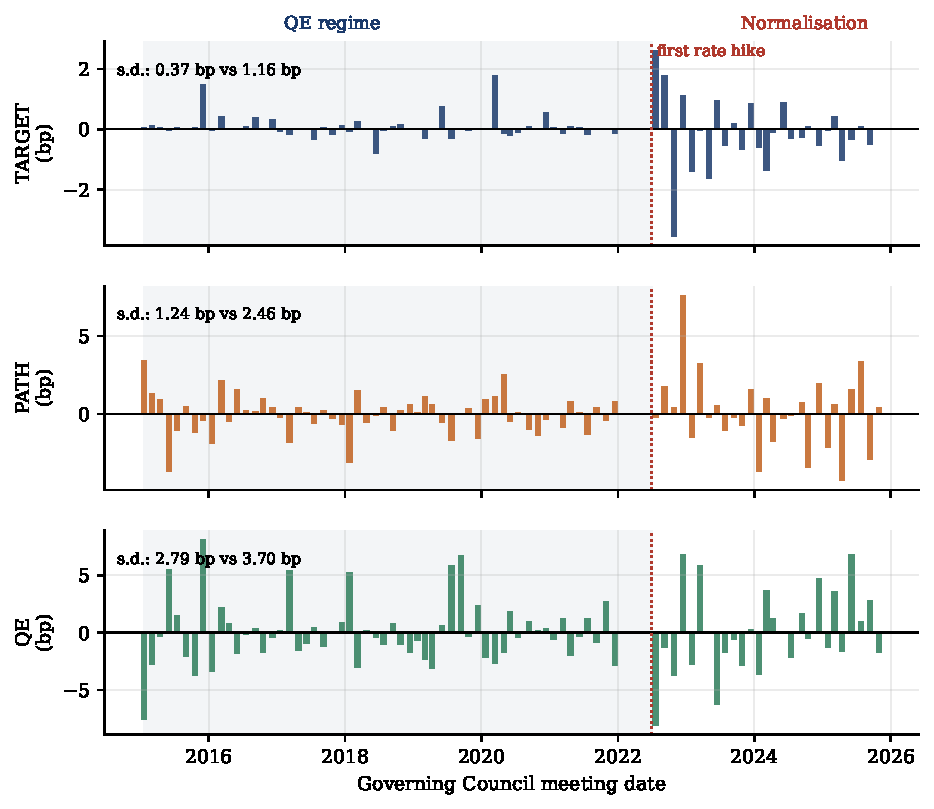
\includegraphics[width=0.95\textwidth]{../output/figures/fig1_factor_series.pdf}
\caption{Estimated policy surprise factors by meeting. The dotted line marks the
July 2022 liftoff. Factor volatility rises in all three dimensions after 2022.}
\label{fig:series}
\end{figure}

\begin{figure}[htbp]\centering
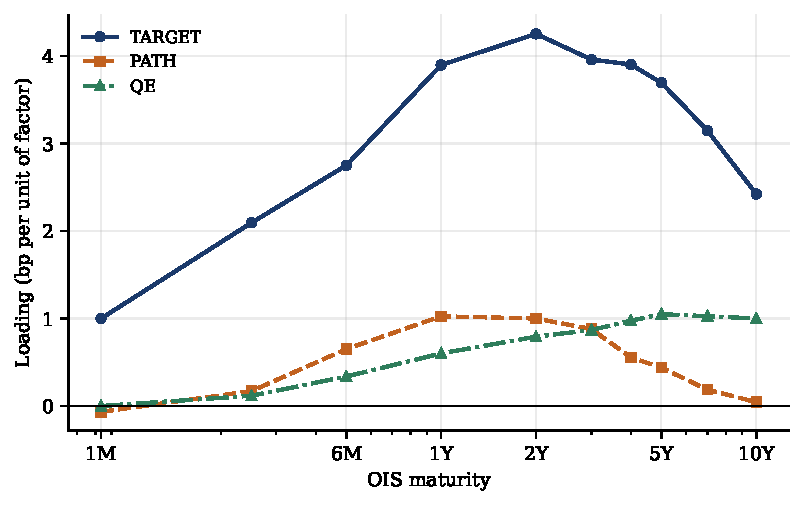
\includegraphics[width=0.75\textwidth]{../output/figures/fig2_loadings.pdf}
\caption{Loading profiles. The shapes are not imposed: only the zero restriction
at one month for the balance-sheet factor is.}
\label{fig:loadings}
\end{figure}

\begin{figure}[htbp]\centering
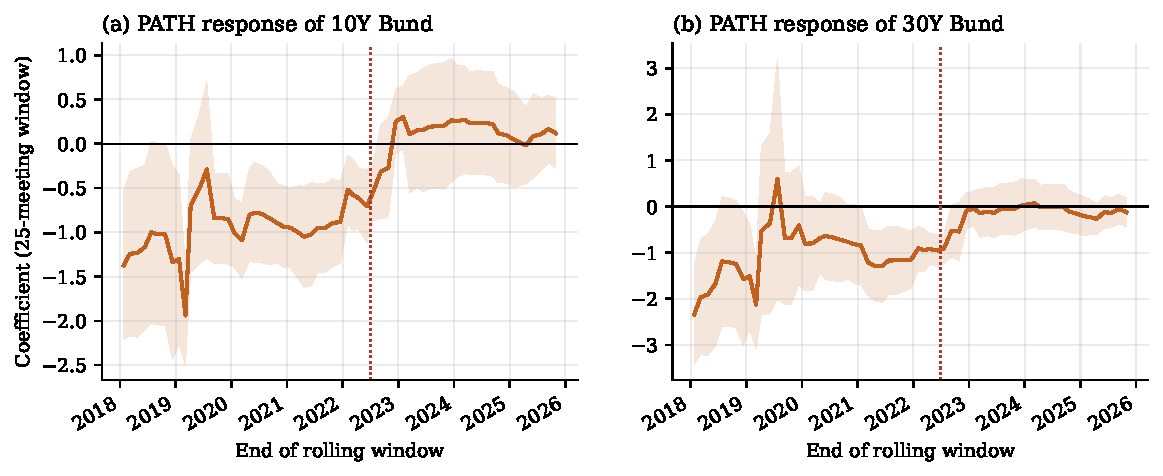
\includegraphics[width=\textwidth]{../output/figures/fig4_rolling.pdf}
\caption{Rolling path coefficients over trailing 25-meeting windows with 90
percent bands, estimated on the sample including the transition semester. Each
point is dated by the last meeting in its window, so a change beginning at the
July 2022 liftoff (dotted line) enters the series gradually and is fully
reflected only once the window has turned over, around early 2023. The
coefficient drifts from roughly $-1$ to zero rather than jumping, which is what
a gradual change in the information content of guidance would produce and what
the regime dummy of equation (\ref{eq:main}) approximates coarsely.}
\label{fig:rolling}
\end{figure}

\begin{figure}[htbp]\centering
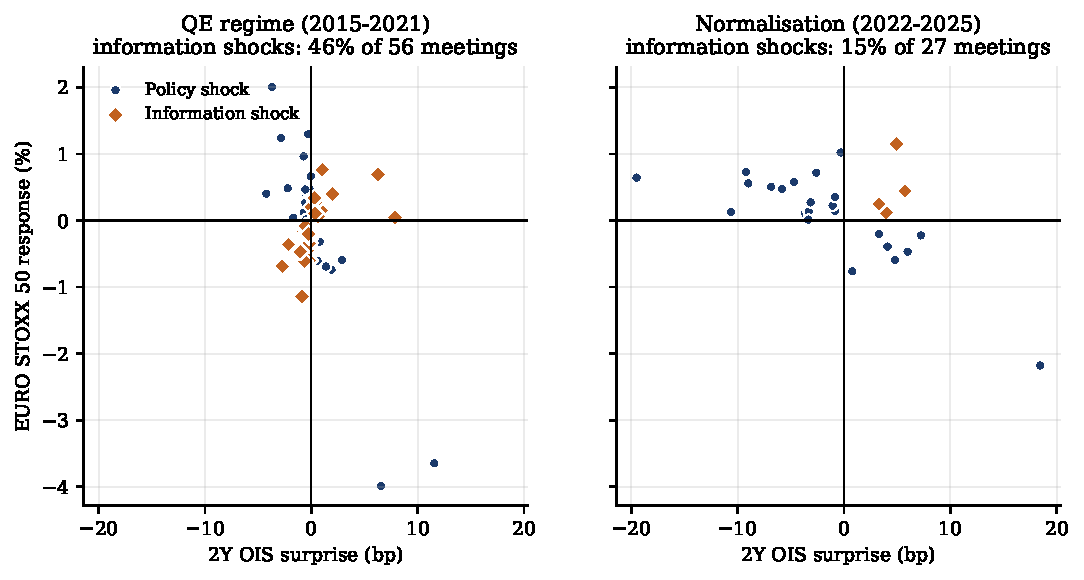
\includegraphics[width=\textwidth]{../output/figures/fig5_information.pdf}
\caption{Interest rate surprise against equity response, by regime, on a common
scale. Points in the shaded co-movement quadrants, where yields and equities
move together, are classified as information shocks. Two features are visible
directly: surprises are several times larger after 2022, and the co-movement
quadrants empty out.}
\label{fig:information}
\end{figure}

\begin{table}[htbp]\centering\footnotesize
\caption{Appendix A1: event dates mis-assigned by a month-first parser}
\fittable{../output/tables/a1_date_audit.tex}
\end{table}

\begin{table}[htbp]\centering\footnotesize
\caption{Appendix A2: baseline responses, all seven outcomes}
\fittable{../output/tables/a8_baseline_full.tex}
\end{table}

\begin{table}[htbp]\centering\footnotesize
\caption{Appendix A3: regime interactions, all seven outcomes}
\fittable{../output/tables/a9_interaction_full.tex}
\begin{minipage}{\textwidth}\footnotesize\vspace{4pt}
The four columns discussed in the text appear in Table \ref{tab:interaction};
this table adds the five-year point, the level factor and curvature.
\end{minipage}
\end{table}

\end{document}
